\section{Evaluation}\label{accept:sec:evaluation}

\edef\codecount#1{%
\ifstrequal{#1}{SQLite3-approx}{1}{\ifstrequal{#1}{SQLite3-endorse}{0}{\ifstrequal{#1}{SQLite3-loc}{145479}{\ifstrequal{#1}{bit-approx}{0}{\ifstrequal{#1}{bit-endorse}{0}{\ifstrequal{#1}{bit-loc}{0}{\ifstrequal{#1}{bitstreams-approx}{0}{\ifstrequal{#1}{bitstreams-endorse}{0}{\ifstrequal{#1}{bitstreams-loc}{0}{\ifstrequal{#1}{blackscholes-approx}{50}{\ifstrequal{#1}{blackscholes-endorse}{10}{\ifstrequal{#1}{blackscholes-loc}{348}{\ifstrequal{#1}{canneal-approx}{91}{\ifstrequal{#1}{canneal-endorse}{8}{\ifstrequal{#1}{canneal-loc}{3144}{\ifstrequal{#1}{ccv-approx}{110}{\ifstrequal{#1}{ccv-endorse}{157}{\ifstrequal{#1}{ccv-loc}{13448}{\ifstrequal{#1}{cpptest-approx}{4}{\ifstrequal{#1}{cpptest-endorse}{0}{\ifstrequal{#1}{cpptest-loc}{29}{\ifstrequal{#1}{fluidanimate-approx}{30}{\ifstrequal{#1}{fluidanimate-endorse}{47}{\ifstrequal{#1}{fluidanimate-loc}{2138}{\ifstrequal{#1}{jean-pierre-approx}{6}{\ifstrequal{#1}{jean-pierre-endorse}{2}{\ifstrequal{#1}{jean-pierre-loc}{1710}{\ifstrequal{#1}{jpeg-approx}{6}{\ifstrequal{#1}{jpeg-endorse}{9}{\ifstrequal{#1}{jpeg-loc}{875}{\ifstrequal{#1}{lib-approx}{0}{\ifstrequal{#1}{lib-endorse}{0}{\ifstrequal{#1}{lib-loc}{0}{\ifstrequal{#1}{msp430-activityrec-approx}{19}{\ifstrequal{#1}{msp430-activityrec-endorse}{5}{\ifstrequal{#1}{msp430-activityrec-loc}{587}{\ifstrequal{#1}{msp430-strawman-approx}{4}{\ifstrequal{#1}{msp430-strawman-endorse}{0}{\ifstrequal{#1}{msp430-strawman-loc}{31}{\ifstrequal{#1}{sobel-approx}{7}{\ifstrequal{#1}{sobel-endorse}{5}{\ifstrequal{#1}{sobel-loc}{154}{\ifstrequal{#1}{strawman-approx}{4}{\ifstrequal{#1}{strawman-endorse}{0}{\ifstrequal{#1}{strawman-loc}{28}{\ifstrequal{#1}{strawman2-approx}{2}{\ifstrequal{#1}{strawman2-endorse}{0}{\ifstrequal{#1}{strawman2-loc}{22}{\ifstrequal{#1}{streamcluster-approx}{51}{\ifstrequal{#1}{streamcluster-endorse}{24}{\ifstrequal{#1}{streamcluster-loc}{1122}{\ifstrequal{#1}{test-sobel-approx}{9}{\ifstrequal{#1}{test-sobel-endorse}{8}{\ifstrequal{#1}{test-sobel-loc}{373}{\ifstrequal{#1}{x264-approx}{300}{\ifstrequal{#1}{x264-endorse}{69}{\ifstrequal{#1}{x264-loc}{22018}{\ifstrequal{#1}{x86-activityrec-approx}{23}{\ifstrequal{#1}{x86-activityrec-endorse}{4}{\ifstrequal{#1}{x86-activityrec-loc}{542}{\ifstrequal{#1}{xapian-approx}{0}{\ifstrequal{#1}{xapian-endorse}{0}{\ifstrequal{#1}{xapian-loc}{88691}{\ifstrequal{#1}{zynq-blackscholes-approx}{50}{\ifstrequal{#1}{zynq-blackscholes-endorse}{10}{\ifstrequal{#1}{zynq-blackscholes-loc}{318}{\ifstrequal{#1}{zynq-fft-approx}{2}{\ifstrequal{#1}{zynq-fft-endorse}{0}{\ifstrequal{#1}{zynq-fft-loc}{111}{\ifstrequal{#1}{zynq-inversek2j-approx}{6}{\ifstrequal{#1}{zynq-inversek2j-endorse}{6}{\ifstrequal{#1}{zynq-inversek2j-loc}{67}{\ifstrequal{#1}{zynq-jmeint-approx}{32}{\ifstrequal{#1}{zynq-jmeint-endorse}{35}{\ifstrequal{#1}{zynq-jmeint-loc}{346}{\ifstrequal{#1}{zynq-sobel-approx}{16}{\ifstrequal{#1}{zynq-sobel-endorse}{7}{\ifstrequal{#1}{zynq-sobel-loc}{356}{\ifstrequal{#1}{zynq-strawman-approx}{1}{\ifstrequal{#1}{zynq-strawman-endorse}{0}{\ifstrequal{#1}{zynq-strawman-loc}{14}{\errmessage{unknown key for codecount: #1}}}}}}}}}}}}}}}}}}}}}}}}}}}}}}}}}}}}}}}}}}}}}}}}}}}}}}}}}}}}}}}}}}}}}}}}}}}}}}}}}}}

\edef\tunestats#1{%
\ifstrequal{#1}{canneal-base-configs}{5}{\ifstrequal{#1}{canneal-composite-configs}{7}{\ifstrequal{#1}{canneal-good-results}{21}{\ifstrequal{#1}{canneal-optimal-results}{11}{\ifstrequal{#1}{canneal-time}{5 minutes}{\ifstrequal{#1}{fluidanimate-base-configs}{20}{\ifstrequal{#1}{fluidanimate-composite-configs}{13}{\ifstrequal{#1}{fluidanimate-good-results}{50}{\ifstrequal{#1}{fluidanimate-optimal-results}{11}{\ifstrequal{#1}{fluidanimate-time}{3 minutes}{\ifstrequal{#1}{msp430-activityrec-base-configs}{4}{\ifstrequal{#1}{msp430-activityrec-composite-configs}{3}{\ifstrequal{#1}{msp430-activityrec-good-results}{7}{\ifstrequal{#1}{msp430-activityrec-optimal-results}{5}{\ifstrequal{#1}{msp430-activityrec-time}{5 minutes}{\ifstrequal{#1}{sobel-base-configs}{6}{\ifstrequal{#1}{sobel-composite-configs}{5}{\ifstrequal{#1}{sobel-good-results}{10}{\ifstrequal{#1}{sobel-optimal-results}{7}{\ifstrequal{#1}{sobel-time}{14 seconds}{\ifstrequal{#1}{streamcluster-base-configs}{23}{\ifstrequal{#1}{streamcluster-composite-configs}{14}{\ifstrequal{#1}{streamcluster-good-results}{18}{\ifstrequal{#1}{streamcluster-optimal-results}{7}{\ifstrequal{#1}{streamcluster-time}{3 minutes}{\ifstrequal{#1}{time-max}{40 minutes}{\ifstrequal{#1}{time-max-app}{zynq-sobel}{\ifstrequal{#1}{time-mean}{9 minutes}{\ifstrequal{#1}{time-min}{14 seconds}{\ifstrequal{#1}{time-min-app}{sobel}{\ifstrequal{#1}{time-msp430-max}{5 minutes}{\ifstrequal{#1}{time-msp430-max-app}{msp430-activityrec}{\ifstrequal{#1}{time-msp430-mean}{5 minutes}{\ifstrequal{#1}{time-msp430-min}{5 minutes}{\ifstrequal{#1}{time-msp430-min-app}{msp430-activityrec}{\ifstrequal{#1}{time-x86-max}{11 minutes}{\ifstrequal{#1}{time-x86-max-app}{x264}{\ifstrequal{#1}{time-x86-mean}{4 minutes}{\ifstrequal{#1}{time-x86-min}{14 seconds}{\ifstrequal{#1}{time-x86-min-app}{sobel}{\ifstrequal{#1}{time-zynq-max}{40 minutes}{\ifstrequal{#1}{time-zynq-max-app}{zynq-sobel}{\ifstrequal{#1}{time-zynq-mean}{19 minutes}{\ifstrequal{#1}{time-zynq-min}{5 minutes}{\ifstrequal{#1}{time-zynq-min-app}{zynq-blackscholes}{\ifstrequal{#1}{x264-base-configs}{23}{\ifstrequal{#1}{x264-composite-configs}{10}{\ifstrequal{#1}{x264-good-results}{17}{\ifstrequal{#1}{x264-optimal-results}{3}{\ifstrequal{#1}{x264-time}{11 minutes}{\ifstrequal{#1}{zynq-blackscholes-base-configs}{2}{\ifstrequal{#1}{zynq-blackscholes-composite-configs}{1}{\ifstrequal{#1}{zynq-blackscholes-good-results}{2}{\ifstrequal{#1}{zynq-blackscholes-optimal-results}{1}{\ifstrequal{#1}{zynq-blackscholes-time}{5 minutes}{\ifstrequal{#1}{zynq-inversek2j-base-configs}{3}{\ifstrequal{#1}{zynq-inversek2j-composite-configs}{2}{\ifstrequal{#1}{zynq-inversek2j-good-results}{2}{\ifstrequal{#1}{zynq-inversek2j-optimal-results}{1}{\ifstrequal{#1}{zynq-inversek2j-time}{12 minutes}{\ifstrequal{#1}{zynq-sobel-base-configs}{6}{\ifstrequal{#1}{zynq-sobel-composite-configs}{2}{\ifstrequal{#1}{zynq-sobel-good-results}{4}{\ifstrequal{#1}{zynq-sobel-optimal-results}{4}{\ifstrequal{#1}{zynq-sobel-time}{40 minutes}{\errmessage{unknown key for tunestats: #1}}}}}}}}}}}}}}}}}}}}}}}}}}}}}}}}}}}}}}}}}}}}}}}}}}}}}}}}}}}}}}}}}}}


\newcommand{\statcols}[1]{
    \codecount{#1-loc} &
    \codecount{#1-approx} &
    \codecount{#1-endorse}
}

\begin{table}
\centering
\begin{tabular}{l l l r r r}
\toprule

Application & Description & Quality Metric &
LOC & \texttt{APPROX} & \texttt{ENDORSE} \\
\cmidrule[\lightrulewidth](r){1-3}
\cmidrule[\lightrulewidth](l){4-6}

\bench{canneal} &
VLSI routing &
% simmedium &
Routing cost &
\statcols{canneal}
\\

\bench{fluidanimate} &
Fluid dynamics &
% simlarge &
Particle distance &
\statcols{fluidanimate}
\\

\bench{streamcluster} & 
Online clustering &
% simlarge &
Cluster center distance &
\statcols{streamcluster}
\\

\bench{x264} & 
Video encoding &
% simmedium &
Structural similarity &
\statcols{x264}
\\

\bench{sobel} &
Sobel filter &
Mean pixel difference &
\statcols{sobel}
\\

\midrule
\bench{zynq-blackscholes} &
Investment pricing &
Mean relative error &
\statcols{zynq-blackscholes}
\\

\bench{zynq-inversek2j} &
Inverse kinematics &
Euclidean distance &
\statcols{zynq-inversek2j}
\\

\bench{zynq-sobel} &
Sobel filter &
Mean pixel difference &
\statcols{zynq-sobel}
\\

\midrule
\bench{msp430-activity} & 
Activity recognition &
Classification rate &
\statcols{msp430-activityrec}
\\

\bottomrule
\end{tabular}
\caption{The approximate applications used in our evaluation. The
final two columns show source code annotation counts.}
\label{accept:table:apps}
\end{table}

We evaluated \sysname's effectiveness at helping programmers
to tune programs.
We collected applications from domains known to be resilient to approximation,
annotated each program using \sysname's feedback mechanisms, and applied the
autotuner to produce relaxed executables.
We examined applications targeting three platforms:
a standard x86 server system,
a mobile SoC augmented with an FPGA for neural acceleration,
and a low-power, embedded sensing device.

\subsection{Applications}

Table~\ref{accept:table:apps} lists the applications we use in this evaluation. Since
there is no standard suite of benchmarks for evaluating approximate-computing
systems, we collect approximable applications from multiple sources,
following the lead of other work in the area~\cite{enerj, npu, benchnn,
qosprof, temam-isca}. Five programs---\bench{canneal}, \bench{fluidanimate},
\bench{streamcluster}, \bench{x264}, and \bench{zynq-blackscholes}---are from the PARSEC
parallel benchmark suite~\cite{parsec}.
They implement physical simulation, machine learning, video, and financial
algorithms.
Another program, \bench{sobel} along
with its ARM port \bench{zynq-sobel}, is an
image convolution kernel implementing the Sobel
filter, a common component of image processing pipelines.
The final program, \bench{msp430-activity}, is an activity-recognition workload that
uses a na\"ive Bayesian classifier to
infer a physical activity from a sequence of accelerometer values on an MSP430
microcontroller~\cite{www:msp430}.

We selected programs for three deployment platforms---a server, a mobile SoC,
and a microcontroller---which we describe in detail below.
In one case, \bench{sobel}, we examine two versions: a conventional
implementation for the server and a version ported to the bare-metal (OS-free)
environment of the SoC.

To evaluate the applications' output accuracy, we
develop application-specific quality metrics as in prior work on approximate
computing~\cite{enerj, green,
qosprof, npu, truffle}.
Table~\ref{accept:table:apps} lists the metric for each program.
In one case,
\bench{fluidanimate}, the benchmark shipped with an output-comparison tool.

We annotated each benchmark by inserting type annotations and
interacting with the compiler's feedback mechanisms to identify fruitful
optimizations.
Table~\ref{accept:table:apps} shows the source code annotation density.
\secref{sec:casestudy} reports qualitatively on our experiences with the
annotation process.

To validate the generality of \sysname's program relaxations, we used one set
of inputs (the \emph{training set}) during autotuning and a distinct input set
(the \emph{testing set}) to evaluate the final speedup and quality loss.

\subsection{Experimental Setup}

\begin{figure}
    \centering
    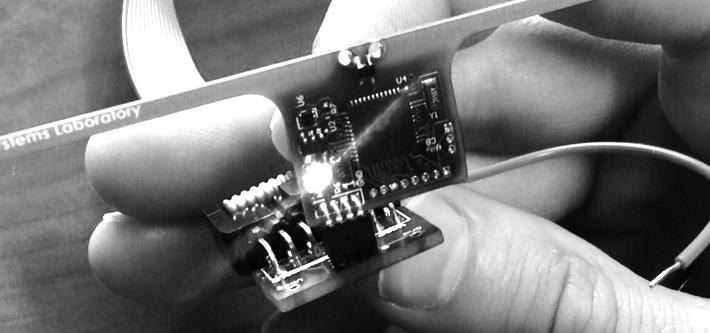
\includegraphics[width=0.8\linewidth]{figs/wisp.jpg}
    \vspace{-1ex}
    \caption{WISP sensing platform~\cite{wisp-transactions}.}
    \label{accept:fig:wispphoto}
\end{figure}

Each application targets one of three evaluation platforms: an x86 server,
an ARM SoC with an integrated FPGA, and an embedded sensing system.
The server platform is a dual-socket, 64-bit, 2.8~GHz Intel Xeon machine with
two-way simultaneous multithreading and 4 GB memory.
During autotuning, we distributed work across a cluster of 20 of these
Xeon machines running Red Hat Enterprise Linux 6.5 with kernel version 2.6.32.
The FPGA-augmented SoC is included to demonstrate the NPU relaxation, which
requires programmable logic.
We implemented the neural-network accelerator (\Sref{sec:accelerator}) on
a Xilinx Zynq-7020 part, which includes a dual-core ARM Cortex-A9 and an FPGA
fabric on a single TSMC 28\,nm die.
Full details on the accelerator implementation can be found in~\cite{snnap}.
Finally,
for the embedded \bench{msp430-activity} workload, we used the
WISP~\cite{wisp-transactions} device depicted in Figure~\ref{accept:fig:wispphoto}. The
WISP incorporates a prototype MSP430FR5969 ``Wolverine'' microcontroller with
2\,KB of SRAM and 64\,KB of nonvolatile ferroelectric RAM (FRAM) along with an
onboard accelerometer.  The WISP can harvest energy from radio waves, but we
powered it via its JTAG interface to ensure reliable, repeatable runs connected
to our test harness.

Only the Zynq platform supports \sysname's neural acceleration optimization.
The server and microcontroller benchmarks used the other two optimizations,
loop perforation and synchronization elision, while the Zynq experiments
explored all three.

We compiled all applications with LLVM's standard \texttt{-O2} optimizations
in addition to \sysname's program relaxations.
%
We measured performance by reading the system clock before and after a
region of interest that excluded the
loading of data files from disk and dumping of results. (This region of
interest was already defined for the PARSEC benchmarks.)
To obtain accurate time measurements, we ran each configuration five times and
averaged the running times.


\subsection{Results}
\label{accept:sec:results}

\begin{figure}[t]
\begin{subfigure}[b]{2.35in}
% GNUPLOT: LaTeX picture with Postscript
\begingroup
\sffamily \footnotesize
  \makeatletter
  \providecommand\color[2][]{%
    \GenericError{(gnuplot) \space\space\space\@spaces}{%
      Package color not loaded in conjunction with
      terminal option `colourtext'%
    }{See the gnuplot documentation for explanation.%
    }{Either use 'blacktext' in gnuplot or load the package
      color.sty in LaTeX.}%
    \renewcommand\color[2][]{}%
  }%
  \providecommand\includegraphics[2][]{%
    \GenericError{(gnuplot) \space\space\space\@spaces}{%
      Package graphicx or graphics not loaded%
    }{See the gnuplot documentation for explanation.%
    }{The gnuplot epslatex terminal needs graphicx.sty or graphics.sty.}%
    \renewcommand\includegraphics[2][]{}%
  }%
  \providecommand\rotatebox[2]{#2}%
  \@ifundefined{ifGPcolor}{%
    \newif\ifGPcolor
    \GPcolorfalse
  }{}%
  \@ifundefined{ifGPblacktext}{%
    \newif\ifGPblacktext
    \GPblacktexttrue
  }{}%
  % define a \g@addto@macro without @ in the name:
  \let\gplgaddtomacro\g@addto@macro
  % define empty templates for all commands taking text:
  \gdef\gplbacktext{}%
  \gdef\gplfronttext{}%
  \makeatother
  \ifGPblacktext
    % no textcolor at all
    \def\colorrgb#1{}%
    \def\colorgray#1{}%
  \else
    % gray or color?
    \ifGPcolor
      \def\colorrgb#1{\color[rgb]{#1}}%
      \def\colorgray#1{\color[gray]{#1}}%
      \expandafter\def\csname LTw\endcsname{\color{white}}%
      \expandafter\def\csname LTb\endcsname{\color{black}}%
      \expandafter\def\csname LTa\endcsname{\color{black}}%
      \expandafter\def\csname LT0\endcsname{\color[rgb]{1,0,0}}%
      \expandafter\def\csname LT1\endcsname{\color[rgb]{0,1,0}}%
      \expandafter\def\csname LT2\endcsname{\color[rgb]{0,0,1}}%
      \expandafter\def\csname LT3\endcsname{\color[rgb]{1,0,1}}%
      \expandafter\def\csname LT4\endcsname{\color[rgb]{0,1,1}}%
      \expandafter\def\csname LT5\endcsname{\color[rgb]{1,1,0}}%
      \expandafter\def\csname LT6\endcsname{\color[rgb]{0,0,0}}%
      \expandafter\def\csname LT7\endcsname{\color[rgb]{1,0.3,0}}%
      \expandafter\def\csname LT8\endcsname{\color[rgb]{0.5,0.5,0.5}}%
    \else
      % gray
      \def\colorrgb#1{\color{black}}%
      \def\colorgray#1{\color[gray]{#1}}%
      \expandafter\def\csname LTw\endcsname{\color{white}}%
      \expandafter\def\csname LTb\endcsname{\color{black}}%
      \expandafter\def\csname LTa\endcsname{\color{black}}%
      \expandafter\def\csname LT0\endcsname{\color{black}}%
      \expandafter\def\csname LT1\endcsname{\color{black}}%
      \expandafter\def\csname LT2\endcsname{\color{black}}%
      \expandafter\def\csname LT3\endcsname{\color{black}}%
      \expandafter\def\csname LT4\endcsname{\color{black}}%
      \expandafter\def\csname LT5\endcsname{\color{black}}%
      \expandafter\def\csname LT6\endcsname{\color{black}}%
      \expandafter\def\csname LT7\endcsname{\color{black}}%
      \expandafter\def\csname LT8\endcsname{\color{black}}%
    \fi
  \fi
  \setlength{\unitlength}{0.0500bp}%
  \begin{picture}(3772.00,3310.00)%
    \gplgaddtomacro\gplbacktext{%
      \csname LTb\endcsname%
      \put(488,704){\makebox(0,0)[r]{\strut{}0$\times$}}%
      \put(488,1203){\makebox(0,0)[r]{\strut{}1$\times$}}%
      \put(488,1702){\makebox(0,0)[r]{\strut{}2$\times$}}%
      \put(488,2201){\makebox(0,0)[r]{\strut{}3$\times$}}%
      \put(488,2700){\makebox(0,0)[r]{\strut{}4$\times$}}%
      \put(488,3199){\makebox(0,0)[r]{\strut{}5$\times$}}%
      \put(670,616){\rotatebox{-45}{\makebox(0,0)[l]{\strut{}\scriptsize{canneal}}}}%
      \put(955,616){\rotatebox{-45}{\makebox(0,0)[l]{\strut{}\scriptsize{fluidanimate}}}}%
      \put(1240,616){\rotatebox{-45}{\makebox(0,0)[l]{\strut{}\scriptsize{streamcluster}}}}%
      \put(1524,616){\rotatebox{-45}{\makebox(0,0)[l]{\strut{}\scriptsize{x264}}}}%
      \put(1809,616){\rotatebox{-45}{\makebox(0,0)[l]{\strut{}\scriptsize{sobel}}}}%
      \put(2094,616){\rotatebox{-45}{\makebox(0,0)[l]{\strut{}\scriptsize{zynq-blackscholes}}}}%
      \put(2379,616){\rotatebox{-45}{\makebox(0,0)[l]{\strut{}\scriptsize{zynq-inversek2j}}}}%
      \put(2663,616){\rotatebox{-45}{\makebox(0,0)[l]{\strut{}\scriptsize{zynq-sobel}}}}%
      \put(2948,616){\rotatebox{-45}{\makebox(0,0)[l]{\strut{}\scriptsize{msp430-activity}}}}%
      \put(3233,616){\rotatebox{-45}{\makebox(0,0)[l]{\strut{}average}}}%
      \put(22,1951){\rotatebox{-270}{\makebox(0,0){\strut{}speedup}}}%
      \put(955,3284){\makebox(0,0){\strut{}\scriptsize 9.4}}%
      \put(2094,3284){\makebox(0,0){\strut{}\scriptsize 10.2}}%
      \put(2379,3284){\makebox(0,0){\strut{}\scriptsize 17.4}}%
    }%
    \gplgaddtomacro\gplfronttext{%
    }%
    \gplbacktext
    \put(0,0){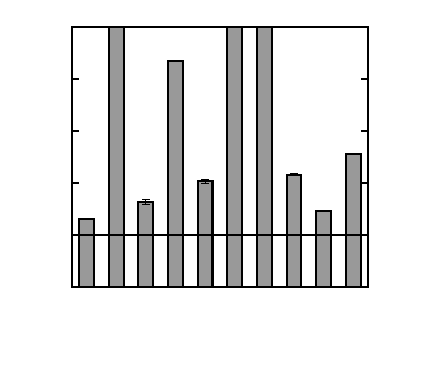
\includegraphics{plots/speedup-all}}%
    \gplfronttext
  \end{picture}%
\endgroup
\vspace{1.5ex}
\caption{Main results (all optimizations)}
\label{accept:fig:speedup-all}
\end{subfigure}
\begin{subfigure}[b]{2.05in}
% GNUPLOT: LaTeX picture with Postscript
\begingroup
\sffamily \footnotesize
  \makeatletter
  \providecommand\color[2][]{%
    \GenericError{(gnuplot) \space\space\space\@spaces}{%
      Package color not loaded in conjunction with
      terminal option `colourtext'%
    }{See the gnuplot documentation for explanation.%
    }{Either use 'blacktext' in gnuplot or load the package
      color.sty in LaTeX.}%
    \renewcommand\color[2][]{}%
  }%
  \providecommand\includegraphics[2][]{%
    \GenericError{(gnuplot) \space\space\space\@spaces}{%
      Package graphicx or graphics not loaded%
    }{See the gnuplot documentation for explanation.%
    }{The gnuplot epslatex terminal needs graphicx.sty or graphics.sty.}%
    \renewcommand\includegraphics[2][]{}%
  }%
  \providecommand\rotatebox[2]{#2}%
  \@ifundefined{ifGPcolor}{%
    \newif\ifGPcolor
    \GPcolorfalse
  }{}%
  \@ifundefined{ifGPblacktext}{%
    \newif\ifGPblacktext
    \GPblacktexttrue
  }{}%
  % define a \g@addto@macro without @ in the name:
  \let\gplgaddtomacro\g@addto@macro
  % define empty templates for all commands taking text:
  \gdef\gplbacktext{}%
  \gdef\gplfronttext{}%
  \makeatother
  \ifGPblacktext
    % no textcolor at all
    \def\colorrgb#1{}%
    \def\colorgray#1{}%
  \else
    % gray or color?
    \ifGPcolor
      \def\colorrgb#1{\color[rgb]{#1}}%
      \def\colorgray#1{\color[gray]{#1}}%
      \expandafter\def\csname LTw\endcsname{\color{white}}%
      \expandafter\def\csname LTb\endcsname{\color{black}}%
      \expandafter\def\csname LTa\endcsname{\color{black}}%
      \expandafter\def\csname LT0\endcsname{\color[rgb]{1,0,0}}%
      \expandafter\def\csname LT1\endcsname{\color[rgb]{0,1,0}}%
      \expandafter\def\csname LT2\endcsname{\color[rgb]{0,0,1}}%
      \expandafter\def\csname LT3\endcsname{\color[rgb]{1,0,1}}%
      \expandafter\def\csname LT4\endcsname{\color[rgb]{0,1,1}}%
      \expandafter\def\csname LT5\endcsname{\color[rgb]{1,1,0}}%
      \expandafter\def\csname LT6\endcsname{\color[rgb]{0,0,0}}%
      \expandafter\def\csname LT7\endcsname{\color[rgb]{1,0.3,0}}%
      \expandafter\def\csname LT8\endcsname{\color[rgb]{0.5,0.5,0.5}}%
    \else
      % gray
      \def\colorrgb#1{\color{black}}%
      \def\colorgray#1{\color[gray]{#1}}%
      \expandafter\def\csname LTw\endcsname{\color{white}}%
      \expandafter\def\csname LTb\endcsname{\color{black}}%
      \expandafter\def\csname LTa\endcsname{\color{black}}%
      \expandafter\def\csname LT0\endcsname{\color{black}}%
      \expandafter\def\csname LT1\endcsname{\color{black}}%
      \expandafter\def\csname LT2\endcsname{\color{black}}%
      \expandafter\def\csname LT3\endcsname{\color{black}}%
      \expandafter\def\csname LT4\endcsname{\color{black}}%
      \expandafter\def\csname LT5\endcsname{\color{black}}%
      \expandafter\def\csname LT6\endcsname{\color{black}}%
      \expandafter\def\csname LT7\endcsname{\color{black}}%
      \expandafter\def\csname LT8\endcsname{\color{black}}%
    \fi
  \fi
  \setlength{\unitlength}{0.0500bp}%
  \begin{picture}(3254.00,3310.00)%
    \gplgaddtomacro\gplbacktext{%
      \csname LTb\endcsname%
      \put(356,704){\makebox(0,0)[r]{\strut{}0$\times$}}%
      \put(356,954){\makebox(0,0)[r]{\strut{}1$\times$}}%
      \put(356,1203){\makebox(0,0)[r]{\strut{}2$\times$}}%
      \put(356,1453){\makebox(0,0)[r]{\strut{}3$\times$}}%
      \put(356,1702){\makebox(0,0)[r]{\strut{}4$\times$}}%
      \put(356,1952){\makebox(0,0)[r]{\strut{}5$\times$}}%
      \put(356,2201){\makebox(0,0)[r]{\strut{}6$\times$}}%
      \put(356,2451){\makebox(0,0)[r]{\strut{}7$\times$}}%
      \put(356,2700){\makebox(0,0)[r]{\strut{}8$\times$}}%
      \put(356,2950){\makebox(0,0)[r]{\strut{}9$\times$}}%
      \put(356,3199){\makebox(0,0)[r]{\strut{}10$\times$}}%
      \put(550,616){\rotatebox{-45}{\makebox(0,0)[l]{\strut{}\scriptsize{canneal}}}}%
      \put(857,616){\rotatebox{-45}{\makebox(0,0)[l]{\strut{}\scriptsize{fluidanimate}}}}%
      \put(1165,616){\rotatebox{-45}{\makebox(0,0)[l]{\strut{}\scriptsize{streamcluster}}}}%
      \put(1473,616){\rotatebox{-45}{\makebox(0,0)[l]{\strut{}\scriptsize{x264}}}}%
      \put(1780,616){\rotatebox{-45}{\makebox(0,0)[l]{\strut{}\scriptsize{sobel}}}}%
      \put(2088,616){\rotatebox{-45}{\makebox(0,0)[l]{\strut{}\scriptsize{zynq-sobel}}}}%
      \put(2396,616){\rotatebox{-45}{\makebox(0,0)[l]{\strut{}\scriptsize{msp430-activity}}}}%
      \put(2703,616){\rotatebox{-45}{\makebox(0,0)[l]{\strut{}average}}}%
    }%
    \gplgaddtomacro\gplfronttext{%
    }%
    \gplbacktext
    \put(0,0){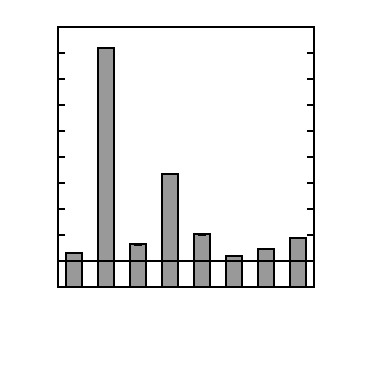
\includegraphics{plots/speedup-loopperf}}%
    \gplfronttext
  \end{picture}%
\endgroup
\vspace{1.5ex}
\caption{Loop perforation}
\label{accept:fig:speedup-loopperf}
\end{subfigure}
\begin{subfigure}[b]{1.15in}
% GNUPLOT: LaTeX picture with Postscript
\begingroup
\sffamily \footnotesize
  \makeatletter
  \providecommand\color[2][]{%
    \GenericError{(gnuplot) \space\space\space\@spaces}{%
      Package color not loaded in conjunction with
      terminal option `colourtext'%
    }{See the gnuplot documentation for explanation.%
    }{Either use 'blacktext' in gnuplot or load the package
      color.sty in LaTeX.}%
    \renewcommand\color[2][]{}%
  }%
  \providecommand\includegraphics[2][]{%
    \GenericError{(gnuplot) \space\space\space\@spaces}{%
      Package graphicx or graphics not loaded%
    }{See the gnuplot documentation for explanation.%
    }{The gnuplot epslatex terminal needs graphicx.sty or graphics.sty.}%
    \renewcommand\includegraphics[2][]{}%
  }%
  \providecommand\rotatebox[2]{#2}%
  \@ifundefined{ifGPcolor}{%
    \newif\ifGPcolor
    \GPcolorfalse
  }{}%
  \@ifundefined{ifGPblacktext}{%
    \newif\ifGPblacktext
    \GPblacktexttrue
  }{}%
  % define a \g@addto@macro without @ in the name:
  \let\gplgaddtomacro\g@addto@macro
  % define empty templates for all commands taking text:
  \gdef\gplbacktext{}%
  \gdef\gplfronttext{}%
  \makeatother
  \ifGPblacktext
    % no textcolor at all
    \def\colorrgb#1{}%
    \def\colorgray#1{}%
  \else
    % gray or color?
    \ifGPcolor
      \def\colorrgb#1{\color[rgb]{#1}}%
      \def\colorgray#1{\color[gray]{#1}}%
      \expandafter\def\csname LTw\endcsname{\color{white}}%
      \expandafter\def\csname LTb\endcsname{\color{black}}%
      \expandafter\def\csname LTa\endcsname{\color{black}}%
      \expandafter\def\csname LT0\endcsname{\color[rgb]{1,0,0}}%
      \expandafter\def\csname LT1\endcsname{\color[rgb]{0,1,0}}%
      \expandafter\def\csname LT2\endcsname{\color[rgb]{0,0,1}}%
      \expandafter\def\csname LT3\endcsname{\color[rgb]{1,0,1}}%
      \expandafter\def\csname LT4\endcsname{\color[rgb]{0,1,1}}%
      \expandafter\def\csname LT5\endcsname{\color[rgb]{1,1,0}}%
      \expandafter\def\csname LT6\endcsname{\color[rgb]{0,0,0}}%
      \expandafter\def\csname LT7\endcsname{\color[rgb]{1,0.3,0}}%
      \expandafter\def\csname LT8\endcsname{\color[rgb]{0.5,0.5,0.5}}%
    \else
      % gray
      \def\colorrgb#1{\color{black}}%
      \def\colorgray#1{\color[gray]{#1}}%
      \expandafter\def\csname LTw\endcsname{\color{white}}%
      \expandafter\def\csname LTb\endcsname{\color{black}}%
      \expandafter\def\csname LTa\endcsname{\color{black}}%
      \expandafter\def\csname LT0\endcsname{\color{black}}%
      \expandafter\def\csname LT1\endcsname{\color{black}}%
      \expandafter\def\csname LT2\endcsname{\color{black}}%
      \expandafter\def\csname LT3\endcsname{\color{black}}%
      \expandafter\def\csname LT4\endcsname{\color{black}}%
      \expandafter\def\csname LT5\endcsname{\color{black}}%
      \expandafter\def\csname LT6\endcsname{\color{black}}%
      \expandafter\def\csname LT7\endcsname{\color{black}}%
      \expandafter\def\csname LT8\endcsname{\color{black}}%
    \fi
  \fi
  \setlength{\unitlength}{0.0500bp}%
  \begin{picture}(1958.00,3310.00)%
    \gplgaddtomacro\gplbacktext{%
      \csname LTb\endcsname%
      \put(356,704){\makebox(0,0)[r]{\strut{}0$\times$}}%
      \put(356,1060){\makebox(0,0)[r]{\strut{}0.2$\times$}}%
      \put(356,1417){\makebox(0,0)[r]{\strut{}0.4$\times$}}%
      \put(356,1773){\makebox(0,0)[r]{\strut{}0.6$\times$}}%
      \put(356,2130){\makebox(0,0)[r]{\strut{}0.8$\times$}}%
      \put(356,2486){\makebox(0,0)[r]{\strut{}1$\times$}}%
      \put(356,2843){\makebox(0,0)[r]{\strut{}1.2$\times$}}%
      \put(356,3199){\makebox(0,0)[r]{\strut{}1.4$\times$}}%
      \put(590,616){\rotatebox{-45}{\makebox(0,0)[l]{\strut{}\scriptsize{fluidanimate}}}}%
      \put(979,616){\rotatebox{-45}{\makebox(0,0)[l]{\strut{}\scriptsize{streamcluster}}}}%
      \put(1367,616){\rotatebox{-45}{\makebox(0,0)[l]{\strut{}average}}}%
    }%
    \gplgaddtomacro\gplfronttext{%
    }%
    \gplbacktext
    \put(0,0){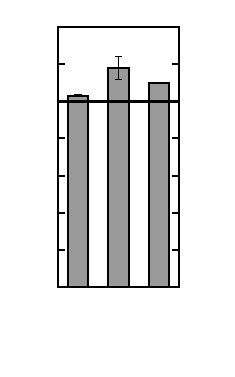
\includegraphics{plots/speedup-desync}}%
    \gplfronttext
  \end{picture}%
\endgroup
\vspace{1.5ex}
\caption{Sync.~elision}
\label{accept:fig:speedup-desync}
\end{subfigure}
\begin{subfigure}[b]{1.3in}
% GNUPLOT: LaTeX picture with Postscript
\begingroup
\sffamily \footnotesize
  \makeatletter
  \providecommand\color[2][]{%
    \GenericError{(gnuplot) \space\space\space\@spaces}{%
      Package color not loaded in conjunction with
      terminal option `colourtext'%
    }{See the gnuplot documentation for explanation.%
    }{Either use 'blacktext' in gnuplot or load the package
      color.sty in LaTeX.}%
    \renewcommand\color[2][]{}%
  }%
  \providecommand\includegraphics[2][]{%
    \GenericError{(gnuplot) \space\space\space\@spaces}{%
      Package graphicx or graphics not loaded%
    }{See the gnuplot documentation for explanation.%
    }{The gnuplot epslatex terminal needs graphicx.sty or graphics.sty.}%
    \renewcommand\includegraphics[2][]{}%
  }%
  \providecommand\rotatebox[2]{#2}%
  \@ifundefined{ifGPcolor}{%
    \newif\ifGPcolor
    \GPcolorfalse
  }{}%
  \@ifundefined{ifGPblacktext}{%
    \newif\ifGPblacktext
    \GPblacktexttrue
  }{}%
  % define a \g@addto@macro without @ in the name:
  \let\gplgaddtomacro\g@addto@macro
  % define empty templates for all commands taking text:
  \gdef\gplbacktext{}%
  \gdef\gplfronttext{}%
  \makeatother
  \ifGPblacktext
    % no textcolor at all
    \def\colorrgb#1{}%
    \def\colorgray#1{}%
  \else
    % gray or color?
    \ifGPcolor
      \def\colorrgb#1{\color[rgb]{#1}}%
      \def\colorgray#1{\color[gray]{#1}}%
      \expandafter\def\csname LTw\endcsname{\color{white}}%
      \expandafter\def\csname LTb\endcsname{\color{black}}%
      \expandafter\def\csname LTa\endcsname{\color{black}}%
      \expandafter\def\csname LT0\endcsname{\color[rgb]{1,0,0}}%
      \expandafter\def\csname LT1\endcsname{\color[rgb]{0,1,0}}%
      \expandafter\def\csname LT2\endcsname{\color[rgb]{0,0,1}}%
      \expandafter\def\csname LT3\endcsname{\color[rgb]{1,0,1}}%
      \expandafter\def\csname LT4\endcsname{\color[rgb]{0,1,1}}%
      \expandafter\def\csname LT5\endcsname{\color[rgb]{1,1,0}}%
      \expandafter\def\csname LT6\endcsname{\color[rgb]{0,0,0}}%
      \expandafter\def\csname LT7\endcsname{\color[rgb]{1,0.3,0}}%
      \expandafter\def\csname LT8\endcsname{\color[rgb]{0.5,0.5,0.5}}%
    \else
      % gray
      \def\colorrgb#1{\color{black}}%
      \def\colorgray#1{\color[gray]{#1}}%
      \expandafter\def\csname LTw\endcsname{\color{white}}%
      \expandafter\def\csname LTb\endcsname{\color{black}}%
      \expandafter\def\csname LTa\endcsname{\color{black}}%
      \expandafter\def\csname LT0\endcsname{\color{black}}%
      \expandafter\def\csname LT1\endcsname{\color{black}}%
      \expandafter\def\csname LT2\endcsname{\color{black}}%
      \expandafter\def\csname LT3\endcsname{\color{black}}%
      \expandafter\def\csname LT4\endcsname{\color{black}}%
      \expandafter\def\csname LT5\endcsname{\color{black}}%
      \expandafter\def\csname LT6\endcsname{\color{black}}%
      \expandafter\def\csname LT7\endcsname{\color{black}}%
      \expandafter\def\csname LT8\endcsname{\color{black}}%
    \fi
  \fi
  \setlength{\unitlength}{0.0500bp}%
  \begin{picture}(2216.00,3310.00)%
    \gplgaddtomacro\gplbacktext{%
      \csname LTb\endcsname%
      \put(356,704){\makebox(0,0)[r]{\strut{}0$\times$}}%
      \put(356,981){\makebox(0,0)[r]{\strut{}2$\times$}}%
      \put(356,1258){\makebox(0,0)[r]{\strut{}4$\times$}}%
      \put(356,1536){\makebox(0,0)[r]{\strut{}6$\times$}}%
      \put(356,1813){\makebox(0,0)[r]{\strut{}8$\times$}}%
      \put(356,2090){\makebox(0,0)[r]{\strut{}10$\times$}}%
      \put(356,2367){\makebox(0,0)[r]{\strut{}12$\times$}}%
      \put(356,2645){\makebox(0,0)[r]{\strut{}14$\times$}}%
      \put(356,2922){\makebox(0,0)[r]{\strut{}16$\times$}}%
      \put(356,3199){\makebox(0,0)[r]{\strut{}18$\times$}}%
      \put(574,616){\rotatebox{-45}{\makebox(0,0)[l]{\strut{}\scriptsize{zynq-blackscholes}}}}%
      \put(930,616){\rotatebox{-45}{\makebox(0,0)[l]{\strut{}\scriptsize{zynq-inversek2j}}}}%
      \put(1285,616){\rotatebox{-45}{\makebox(0,0)[l]{\strut{}\scriptsize{zynq-sobel}}}}%
      \put(1641,616){\rotatebox{-45}{\makebox(0,0)[l]{\strut{}average}}}%
    }%
    \gplgaddtomacro\gplfronttext{%
    }%
    \gplbacktext
    \put(0,0){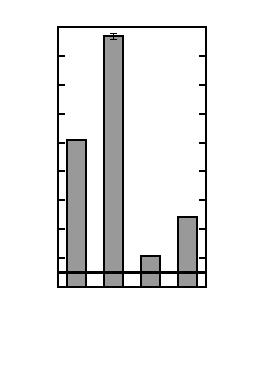
\includegraphics{plots/speedup-npu}}%
    \gplfronttext
  \end{picture}%
\endgroup
\vspace{1.5ex}
\caption{Neural acceleration}
\label{accept:fig:speedup-npu}
\end{subfigure}
\caption{Speedup for each application, including all
optimizations (a) and each optimization in isolation (b--d).}
\label{accept:fig:performance}
\end{figure}

\begin{table}
\centering
\begin{tabular}{l r r r r r r}
\toprule
Application & Sites & Composites & Total & Optimal & Error & Speedup \\
\midrule
\bench{canneal} & 5 & 7 & 32 & 11 & 1.5--15.3\% & 1.1--1.7$\times$\\
\bench{fluidanimate} & 20 & 13 & 82 & 11 & $<$0.1\% & 1.0--9.4$\times$\\
\bench{streamcluster} & 23 & 14 & 66 & 7 & $<$0.1--12.8\% & 1.0--1.9$\times$\\
\bench{x264} & 23 & 10 & 94 & 3 & $<$0.1--0.8\% & 1.0--4.3$\times$\\
\bench{sobel} & 6 & 5 & 21 & 7 & $<$0.1--26.7\% & 1.1--2.0$\times$\\
\bench{zynq-blackscholes} & 2 & 1 & 5 & 1 & 4.3\% & 10.2$\times$\\
\bench{zynq-inversek2j} & 3 & 2 & 10 & 1 & 8.9\% & 17.4$\times$\\
\bench{zynq-sobel} & 6 & 2 & 27 & 4 & 2.2--6.2\% & 1.1--2.2$\times$\\
\bench{msp430-activity} & 4 & 3 & 15 & 5 & $<$0.1\% & 1.5$\times$\\


\bottomrule
\end{tabular}
\caption{Tuning statistics and resulting optimal configurations for each benchmark.}
\label{accept:table:stats}
\end{table}

Figure~\ref{accept:fig:speedup-all} plots the speedup (versus precise execution) of the
best-performing relaxed versions that \sysname found for each application with
output error under 10\%.
Speedups in the figure range from \result{speedup-min}
(\bench{\result{speedup-min-app}}) to \result{speedup-max}
(\bench{\result{speedup-max-app}}) with
a harmonic mean of \result{speedup-x86-mean} across all three platforms.

Figure~\ref{accept:fig:performance} shows the speedup for relaxed versions with only
one type of optimization enabled.
Not every optimization applies to every benchmark: notably, neural
acceleration applies only to the Zynq benchmarks, and synchronization elision
applies only to the two benchmarks that use fine-grained lock- and
barrier-based synchronization.
Loop perforation is the most general relaxation strategy and achieves a
\result{speedup-loopperf-mean} average speedup across
\result{speedup-loopperf-count} of the benchmarks.
Synchronization elision applies to \bench{fluidanimate} and
\bench{streamcluster}, for which it offers speedups of
3\%  % NB: HARD-CODED! (sigfigs)
and \result{speedup-desync-streamcluster} respectively.
The optimization reduces lock contention, which does not dominate the running
time of these benchmarks.
Neural acceleration offers the largest speedups, ranging from
\result{speedup-npu-min} for \bench{\result{speedup-npu-min-app}}
to
\result{speedup-npu-max} for \bench{\result{speedup-npu-max-app}}.

\sysname's feedback system explores a two-dimensional trade-off space between
output quality and performance. For each benchmark, \sysname reports
Pareto-optimal configurations rather than a single ``best'' relaxed executable;
the
programmer can select the configuration that strikes the best
quality--performance balance for a particular deployment.
%
Table~\ref{accept:table:stats} shows the range of output error rates and speedups in
the frontiers for our benchmarks.
%
We highlight \bench{canneal} as an example.
For this program, \sysname identifies \result{pareto-canneal-count}
configurations with output error ranging from \result{pareto-canneal-err-min} to
\result{pareto-canneal-err-max} and speedup ranging from
\result{pareto-canneal-speedup-min} to \result{pareto-canneal-speedup-max}.
Using this Pareto frontier output, the developer can choose a
configuration with a lower speedup in error-sensitive situations or a
more aggressive \result{pareto-canneal-speedup-max} speedup if higher
error is considered acceptable for a
deployment.

One benchmark, \bench{fluidanimate}, exhibits especially low error even under
aggressive optimization;
the configuration with the best speedup,
which removed two locks and perforated nine loops, had
overall error (change in final particle positions) under $0.00001$\%.  For
\bench{msp430-activity}, error remained at $0$\% in all acceptable
configurations.

\paragraph{Autotuner characterization.}

Table~\ref{accept:table:stats} shows
the number of relaxation opportunities (labeled \term{sites}), the number of
composite configurations considered, the total number of configurations
explored (including parameter-tuning configurations),
and the number of optimal configurations on the output Pareto frontier
for each benchmark.
For \bench{streamcluster}, a moderately sized benchmark by code size,
exhaustive exploration of the \tunestats{streamcluster-base-configs}
optimizations would
have required more than 8 million executions;
instead, \sysname's search heuristic considered only
\tunestats{streamcluster-composite-configs} composites
to produce \tunestats{streamcluster-optimal-results} optimal configurations.

\sysname's heuristics help make its profiling step palatable.
On our 20-node evaluation cluster for the server applications, the total end-to-end optimization time was
typically within a few minutes: times ranged from \tunestats{time-x86-min}
(\bench{\tunestats{time-x86-min-app}}) to \tunestats{time-x86-max}
(\bench{\tunestats{time-x86-max-app}}) with an
average of \tunestats{time-x86-mean}.
Tuning for the Zynq and MSP430 platforms was not parallelized and took
\tunestats{time-zynq-mean} on average and
\tunestats{time-msp430-mean}, respectively.

\paragraph{Accelerator power and energy.}
We measured power consumption on the Zynq SoC, including its FPGA and DRAM,
using a Texas Instruments UCD9240 power supply controller while executing each
benchmark in a loop to reach a steady state.
Compared to baseline ARM-core--only execution in which the FPGA is
not programmed and inactive, power overheads range from
from 8.6\% (\bench{zynq-sobel})
to 22.6\% (\bench{zynq-blackscholes}).
The \bench{zynq-sobel} benchmark exhibits
lower power overhead because a larger percentage
of the program executes on the CPU, putting less load on the FPGA.
When we account for the performance gains, energy savings range from 2$\times$ (\bench{zynq-sobel}) to 15.7$\times$ (\bench{zynq-inversek2j}).

% The \bench{zynq-blackscholes} benchmark
% exhibits the opposite balance, with most execution offloaded to the accelerator;
% the accelerator's performance improvements dominate these power
% overheads, so total energy remains less than the baseline. Overall, 


\subsection{Experiences}
\label{accept:sec:casestudy}

This section
reports qualitatively on our experiences using \sysname to optimize the benchmarks.
The programmers included three undergraduate researchers, all of whom were
beginners with C and C++ and new to approximate computing,
as well as graduate students familiar with the field.


\paragraph{Quality metrics.}
The first step in tuning a program with \sysname is to write a quality metric.
In some cases, the program included code to assess output quality.
For each remaining
case, the programmer wrote a simple Python program (54 lines at most) to parse the
program's output and compute the difference between two outputs.

Like any specification, a quality metric can be subtle to write correctly.
Although it was not an intended use case, programmers found \sysname's dynamic feedback to be helpful in debugging quality metrics.
In one instance, \sysname reported suspiciously low error for some
configurations; these results revealed a quality metric that was ignoring
certain missing values in the output and was therefore too permissive.


\paragraph{Initial and iterated annotations.}
One option when annotating a program for \sysname is to first analyze an
unannotated program to enumerate all potential optimization sites.
However, the programmers preferred
to
provide an initial annotation set by finding the ``core''
approximable data in the program---e.g., the vector coordinates in
\bench{streamcluster} or the pixels in \bench{sobel}. With this data marked as
approximate, the type
checker reports errors when this data flows into variables that are not yet
marked; for each such error, programmers decided whether to add another \lil{APPROX}
annotation or to stop the flow of approximation with an \lil{ENDORSE}
annotation.

Next, programmers expanded the annotation set to enable more optimizations.
Using \sysname's analysis log (Section~\ref{accept:sec:feedback}), they looked for
optimizations that could \emph{almost} apply---those that indicated only a
small number of blockers.

A persistent consideration was the need to balance effort with potential
reward.  The programmers focused their attention on parts of the code
most likely to provide good quality--efficiency trade-offs.
In some cases, it was helpful to take ``shortcuts'' to program relaxations to
test their viability before making them safe.
If the programmer was unsure whether a particular lock in a
program was contended, for example, it was useful to try eliding that lock to
see whether it offered any speedup.
Programmers used the \annpermit annotation
\emph{temporarily} for an experiment and then, if the optimization proved
beneficial, removed the escape-hatch annotation and added the safer
\lil{APPROX} and \lil{ENDORSE} annotations.

These experiences highlighted the dual importance of both static and dynamic
feedback in \sysname.
Especially when the programmer is unfamiliar with the application's
architecture, the static type errors and conservative \precisepurity analysis
helped highlight unexpected interactions between components.
However, test runs were critical in discovering whether a
given subcomputation is important to an algorithm, either in terms of
performance or output accuracy.
Both components help alleviate the ``manual labor'' otherwise necessary to
reason about hidden program effects or repeatedly invoke and analyze
measurement runs.

\paragraph{Code navigation and heuristics.}
For large programs, programmers reported a need to balance their time
between learning the application's architecture and trying new
optimizations.
(We anticipate that a different strategy would be appropriate when the
programmer is already familiar with the code before annotation.)
One programmer used a call-graph visualizer to find code closely related
to the main computation.
In general, more modular code was easier to annotate: when effects are
encapsulated, the volume of code related to an optimization is smaller
and annotations are more local.

Programmers relied on \sysname's analysis feedback for hints about where time
would be best spent.
They learned to scan for and ignore reports involving memory allocation
or system calls, which are rarely fruitful approximation opportunities.
Relaxation sites primarily involved with large data arrays were typically good
targets.

\paragraph{Encapsulating precise systems programming.}
The ``escape hatches'' from \sysname's safety analysis were crucial for
low-level systems code.
In \bench{msp430-activity}, a routine manipulates memory-mapped registers to read
from an accelerometer. The pointers involved in
communicating with the memory-mapped peripheral are necessarily precise, but
the reading itself is approximate and safe to relax.
The \annpermit escape hatch enabled its optimization.
This annotation suggests a pattern in systems programming: the language's
last-resort annotations can communicate approximation information about
opaque low-level code to \sysname.

\paragraph{Self-checking code.}
The complementary escape hatch, \annforbid, was useful for one specific
pattern: when benchmarks include code to evaluate their own quality. For
example, \bench{x264} computes a standard image quality metric and
\bench{canneal} evaluates the total design fitness at every iteration.
Programmers used \annforbid to ensure that this code, despite involving
approximate data, was never corrupted.
